\pagebreak
\section{Results and Discussion}

\label{sec:results}


\begin{table}[h!]
    \centering
    \begin{tabular}{ |l|c|c|c|c|c| } 
        \hline
        metrics & run1 & run2 & run3 & run4 & run5 \\ \hline
        num\_q & 657 & 669 & 669 & 667 & 667 \\ \hline
        num\_ret & 646525 & 658446 & 658347 & 652222 & 657903 \\ \hline
        num\_rel & 2550 & 2611 & 2611 & 2603 & 2600 \\ \hline
        num\_rel\_ret & 1772 & 2182 & 2191 & 1866 & 2232 \\ \hline
        map & 0.1307 & 0.2022 & 0.2335 & 0.1856 & 0.2351 \\ \hline
        gm\_map & 0.0117 & 0.046 & 0.061 & 0.0239 & 0.0629 \\ \hline
        Rprec & 0.1041 & 0.1697 & 0.1989 & 0.1654 & 0.2022 \\ \hline
        bpref & 0.3142 & 0.3734 & 0.3869 & 0.3466 & 0.3861 \\ \hline
        recip\_rank & 0.2436 & 0.3287 & 0.3891 & 0.3441 & 0.3945 \\ \hline
        iprec\_at\_recall\_0.00 & 0.2553 & 0.3499 & 0.4134 & 0.3584 & 0.4182 \\ \hline
        iprec\_at\_recall\_0.20 & 0.2387 & 0.3324 & 0.3873 & 0.3353 & 0.3927 \\ \hline
        iprec\_at\_recall\_0.40 & 0.1441 & 0.2316 & 0.2732 & 0.2066 & 0.2716 \\ \hline
        iprec\_at\_recall\_0.60 & 0.0965 & 0.1786 & 0.1996 & 0.1388 & 0.2014 \\ \hline
        iprec\_at\_recall\_0.80 & 0.0628 & 0.1178 & 0.1311 & 0.0887 & 0.1295 \\ \hline
        iprec\_at\_recall\_1.00 & 0.0525 & 0.0954 & 0.1031 & 0.0704 & 0.1028 \\ \hline
        P\_10 & 0.0848 & 0.1296 & 0.1435 & 0.1126 & 0.1432 \\ \hline
        P\_100 & 0.0186 & 0.0256 & 0.0268 & 0.0222 & 0.0268 \\ \hline
        P\_1000 & 0.0027 & 0.0033 & 0.0033 & 0.0028 & 0.0033 \\ \hline
        recall\_10 & 0.2166 & 0.3352 & 0.367 & 0.2849 & 0.3621 \\ \hline
        recall\_100 & 0.4718 & 0.6426 & 0.6714 & 0.5536 & 0.6723 \\ \hline
        recall\_1000 & 0.6816 & 0.8192 & 0.8218 & 0.7004 & 0.8392 \\ \hline
        infAP & 0.1307 & 0.2022 & 0.2335 & 0.1856 & 0.2351 \\ \hline
        gm\_bpref & 0.0152 & 0.0387 & 0.0405 & 0.022 & 0.038 \\ \hline
        utility & -978.6621 & -977.701 & -977.5262 & -972.2489 & -979.6687 \\ \hline
        ndcg & 0.2719 & 0.3655 & 0.3924 & 0.3291 & 0.3982 \\ \hline
        ndcg\_rel & 0.236 & 0.3119 & 0.3416 & 0.2939 & 0.3471 \\ \hline
        Rndcg & 0.1708 & 0.2387 & 0.2657 & 0.2271 & 0.2714 \\ \hline
        ndcg\_cut\_5 & 0.1285 & 0.1908 & 0.2232 & 0.1854 & 0.2269 \\ \hline
        ndcg\_cut\_10 & 0.1609 & 0.2426 & 0.2739 & 0.2227 & 0.2758 \\ \hline
        ndcg\_cut\_100 & 0.2351 & 0.3349 & 0.3652 & 0.3016 & 0.3678 \\ \hline
        ndcg\_cut\_1000 & 0.2719 & 0.3655 & 0.3924 & 0.3291 & 0.3982 \\ \hline
        map\_cut\_10 & 0.1046 & 0.1665 & 0.1975 & 0.1556 & 0.1993 \\ \hline
        map\_cut\_100 & 0.1284 & 0.2 & 0.2315 & 0.1836 & 0.2328 \\ \hline
        map\_cut\_1000 & 0.1307 & 0.2022 & 0.2335 & 0.1856 & 0.2351 \\ \hline
        
    \end{tabular}
    \caption{English results from TREC eval}
    \label{table:results}
\end{table}




\begin{figure}[h!]
    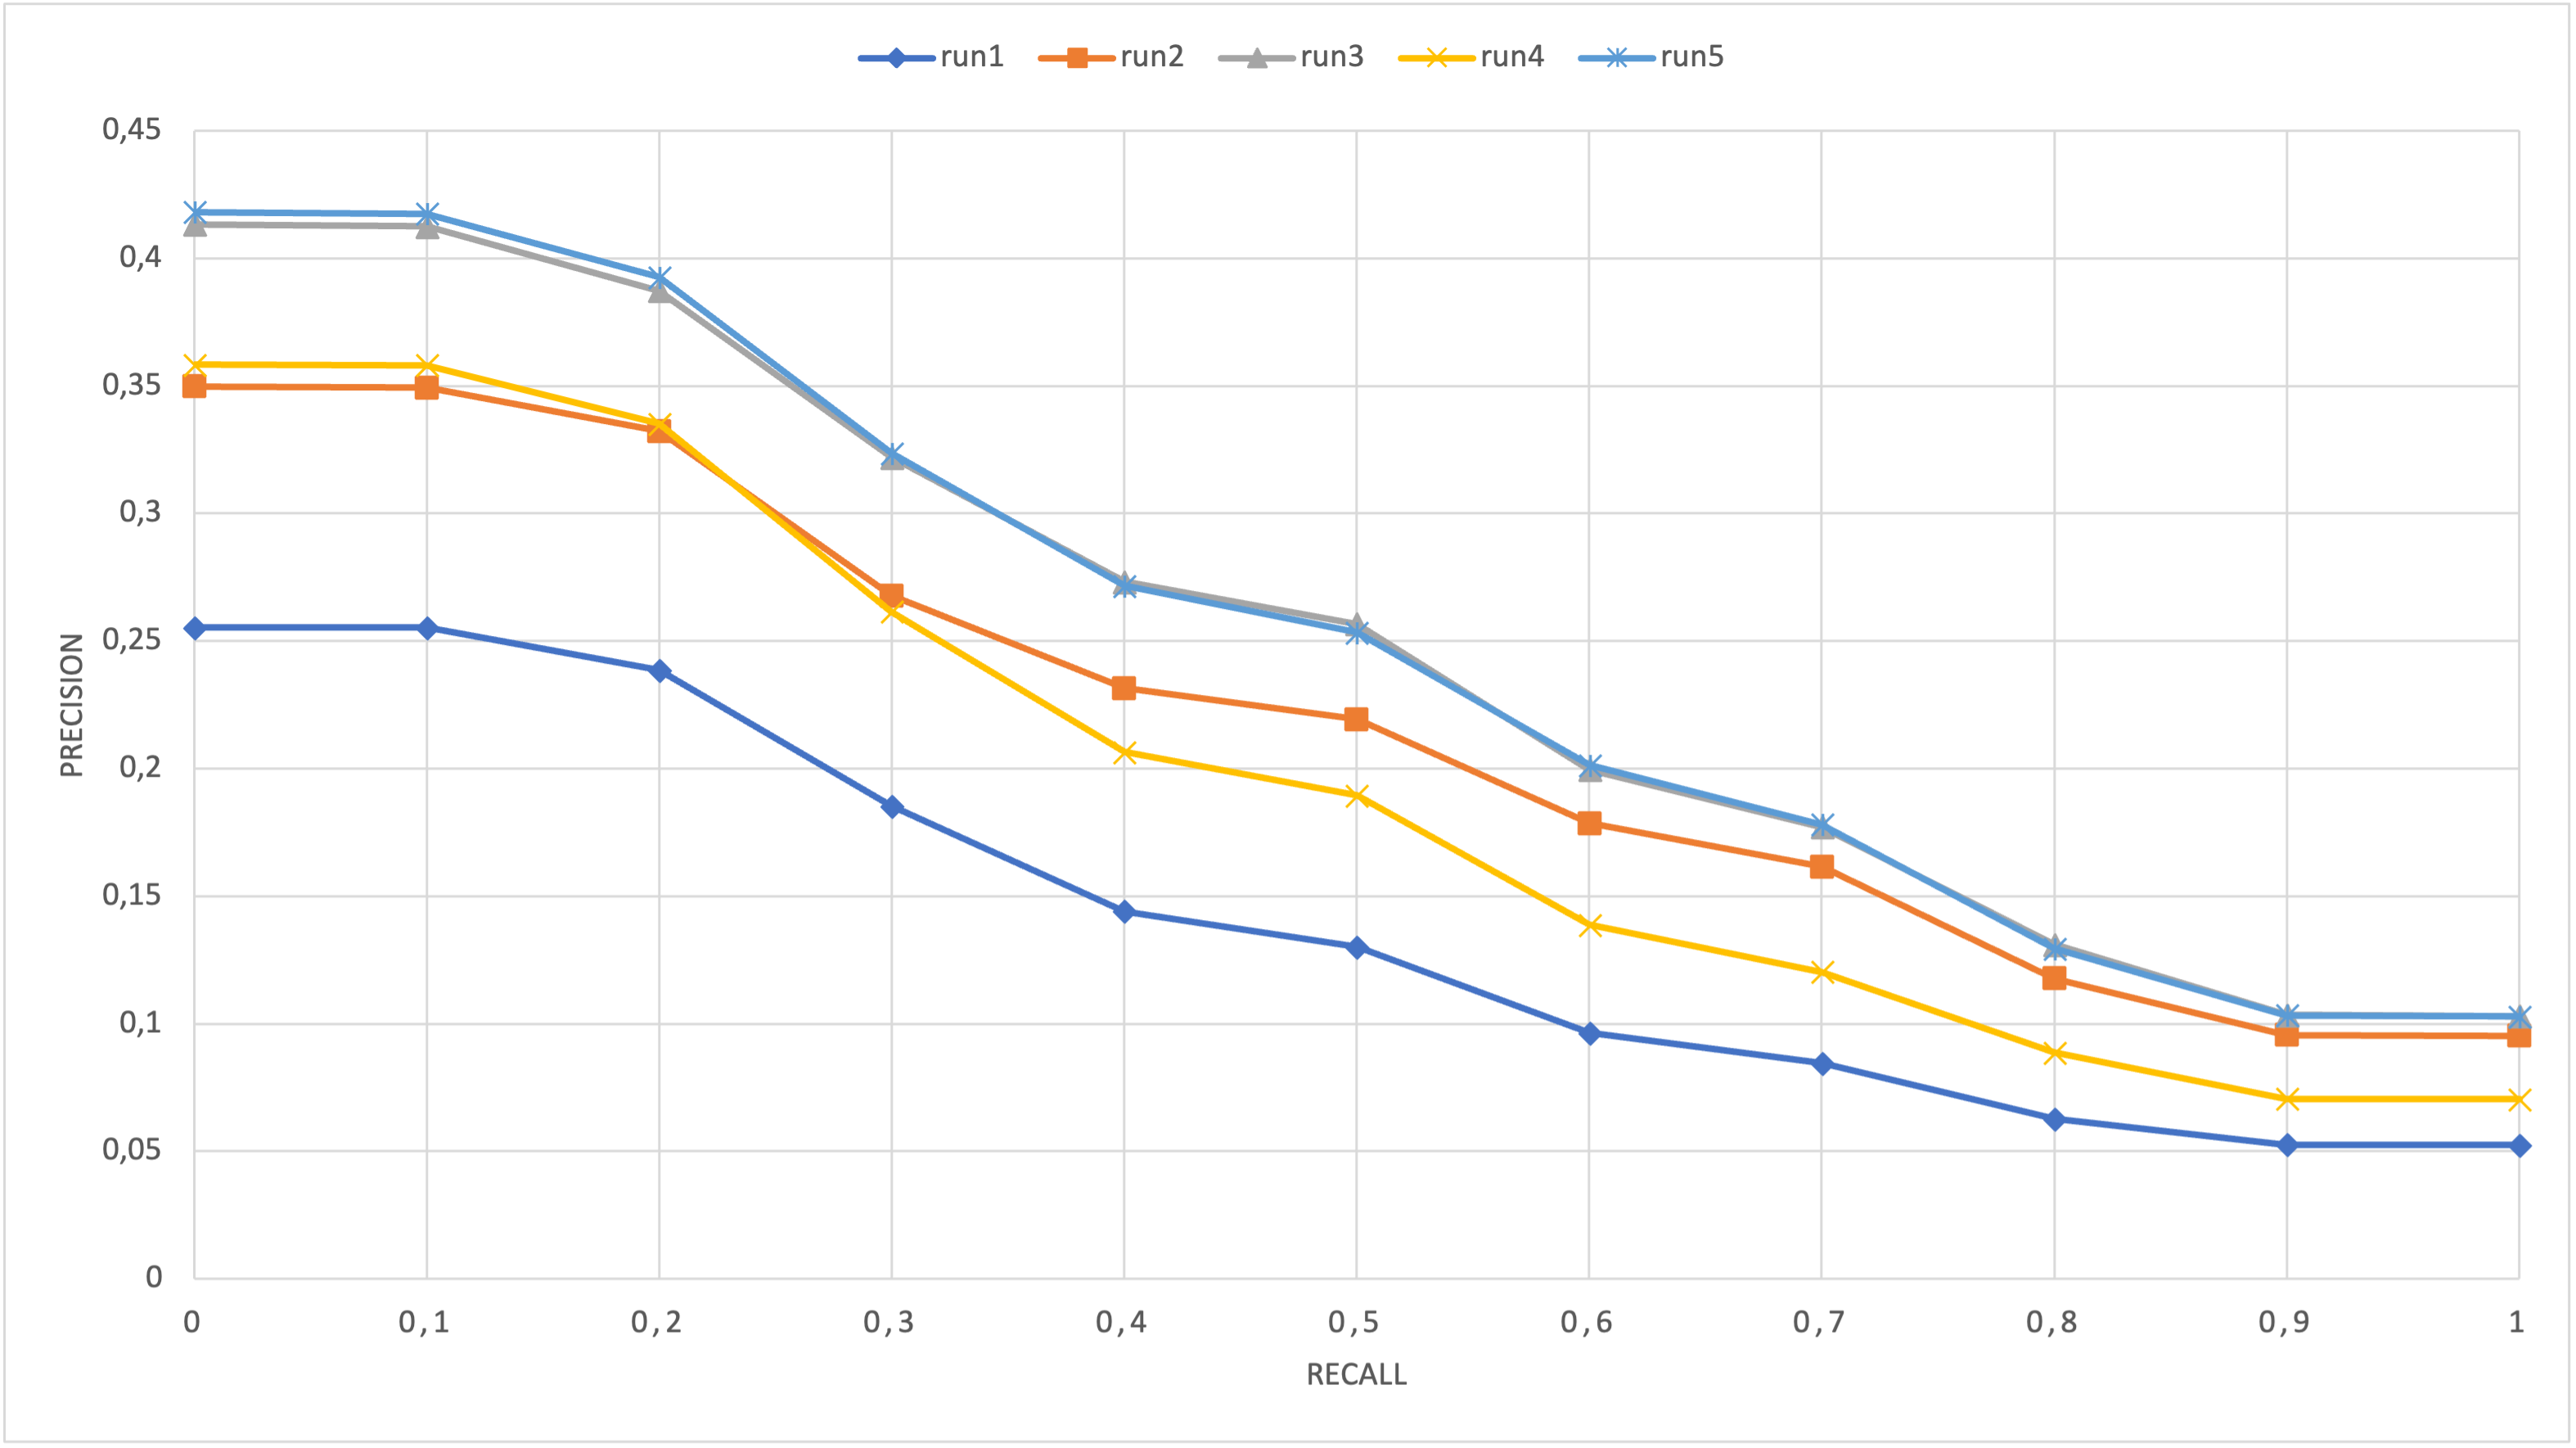
\includegraphics[width=\textwidth]{figure/PRgraph.png}
    \caption{Recall and precision graph}
    \label{fig:recallPrecision}
  \end{figure}
In this Section, we provide some of the most relevant results we got during the development phase.
We are considering five principal milestones that, within many different trials, led us to improve significantly our \ac{MAP} score and the overall number of relevant documents actually retrieved.

First of all, given that we were provided with two different versions of the same document's \textit{corpora}, our first idea was to try the English version.\\ 
We noticed that the best combination of basic \ac{IR} tools was to use the \textit{Porter} Stemmer \cite{solrporterstemfilter}, a length filter from 1 to 10, and a list of stop-word composed by some standard terms and more from the top 600 extracted from the index.
The very first big milestone, that helped us to increment the \ac{MAP} of around 3 points, from 10.1\% to 13.1\%, was the \textit{JavaScript} code cleaner since we noticed by inspection that many documents were having these types of scripts inside.\\
Always by inspecting some documents and queries, and also considering that the original collection was the French version (translated then in English), we observed that the translation was very poor: by switching to French
by just cleaning the \textit{JS} code and some other minor cleaning tools, without even using an adequate stop-list and a correct stemmer for the French language, the \ac{MAP} was increasing by +5\%. \\
2 more \ac{MAP} points were achieved with a stop list built for French in the same way we did previously for English, the \textit{FrenchLightStemFilter}~\cite{solrfrenchlightstemfilter} as stemmer, and moving the length filter from 2 to 15 (as we noticed French tends to have longer words). \\
We tried some \ac{NLP} techniques for English to see if there were improvements, and in this case, apply them to our main implementation for French with an appropriate model. The obtained results were not interesting, and also the computing time was definitely too costly. In particular, we tried to use Solr OpenNLP Part of Speech Filter \cite{solropennlpposfilter} using the \textit{en-pos-maxent} \ac{PoS} tagger provided by \textit{OpenNLP}. 
Another approach we tried and that carried an improvement was to use \textit{Query expansion}: first we used some generative text models to expand our queries, then we decided to weight different query scores by boosting the original one linearly with respect to the number
%of expansion used, and without boosting the expansion: this carried to us an extra MAP point.
of expansion used. This made us gain an extra \ac{MAP} point.

\newpage
\enlargethispage{4\baselineskip}
\begin{figure}[h!]
    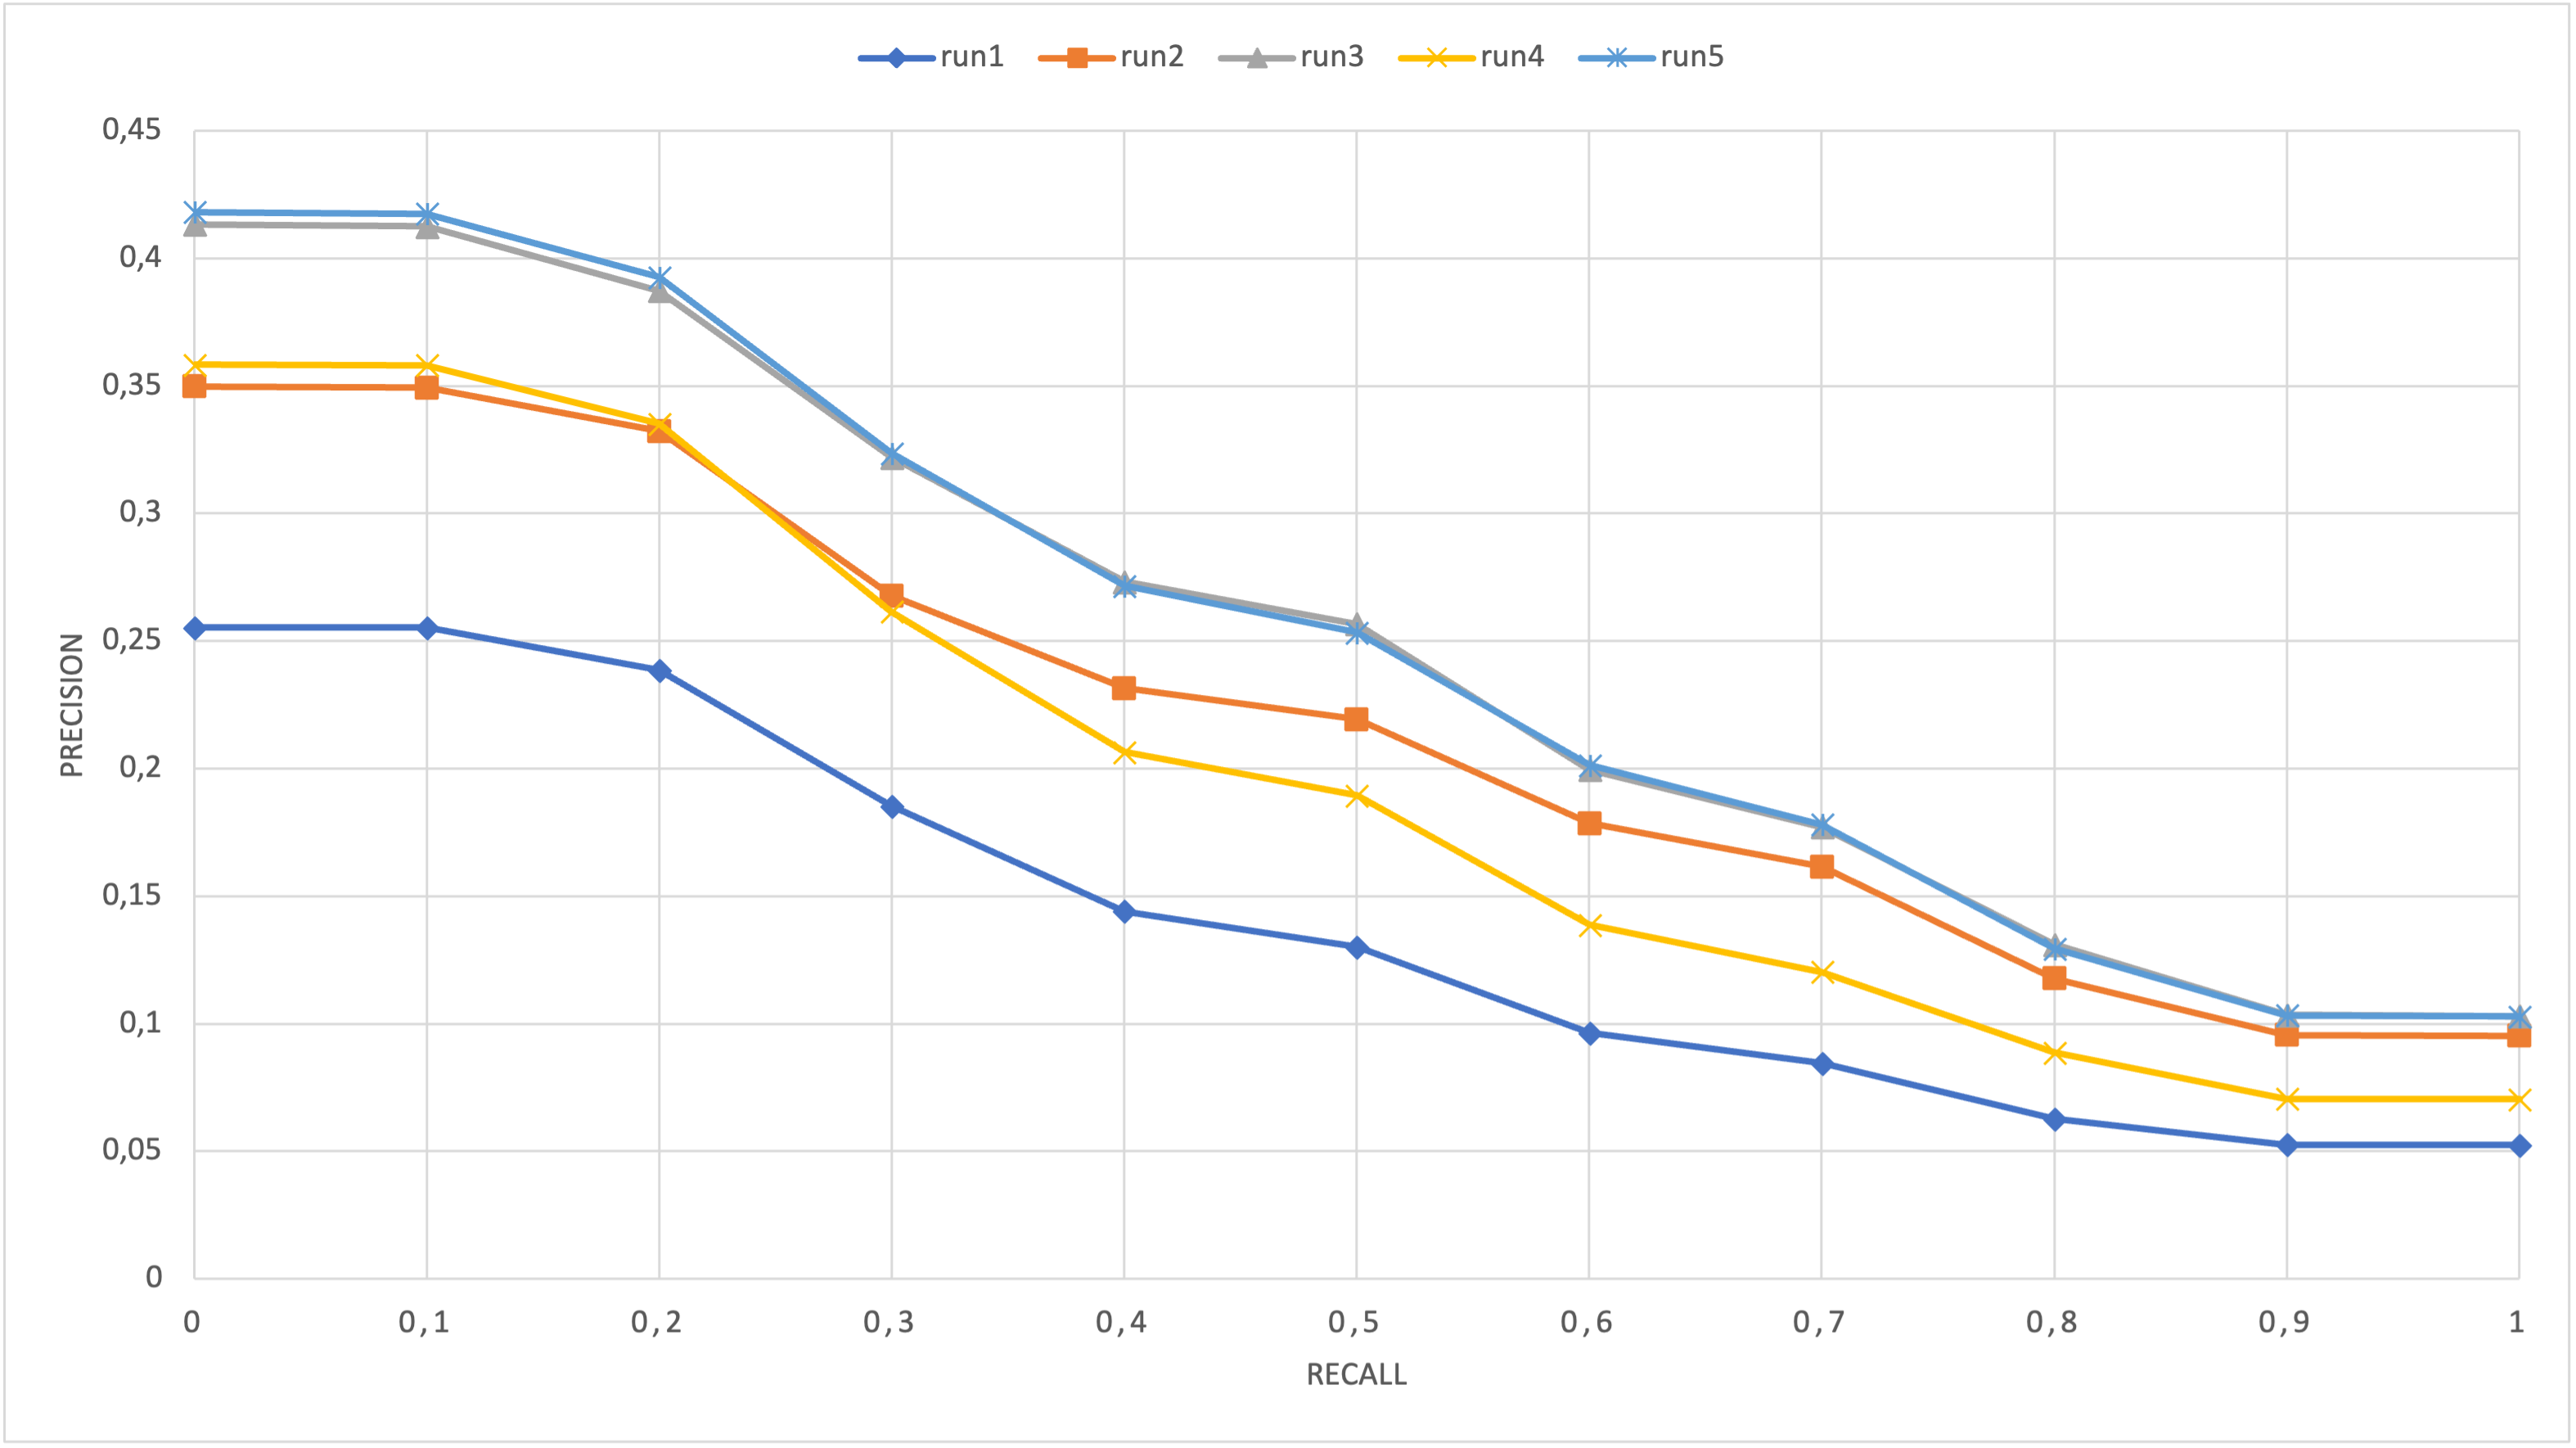
\includegraphics[width=\textwidth]{figure/PRgraph.png}
    \caption{Recall and precision graph}
    \label{fig:recallPrecision}
\end{figure}

We try to generate the embeddings for each document based on word2vector, we use a pre-trained word2vec model \textit{frWac\_no\_postag\_no\_phrase\_500\_cbow\_cut100}~\cite{fauconnier_2015} for French. Then we calculate the embedding for each document and index them as KnnFloatVectorField in Lucene and use KnnFloatVectorQuery \cite{lucene-knnvectorfield} for searching the query to find the \textit{k} nearest documents to the target vector according to the vectors in the given field, but the results (overall \ac{MAP} ~0.08) were not satisfying, being worse than the case of indexing and searching without embeddings.
\newline
We then tried to combine different similarities rather than using the classic \textit{BM25Similarity}: we tried to use the Lucene \textit{MultiSimilarity} \cite{lucenemultisimilarity}, that allows combining the score of two or more similarity scores, but it does not allow to
tune the weights. Then, we tried to reimplement the \textit{MultiSimilarity} class with tuning options, but the results were always lower than the standard \textit{BM25Similarity}. Some minor improvements came up by fine-tuning the document-length
normalization \textit{b} parameter and the term frequency component \textit{k1} parameter of the \textit{BM25Similarity}.
\newline
The last main implementation we did, was to use some \textit{Re-ranking} techniques to improve the results of the first retrieval phase.
We tried to use the \textit{SBERT} model~\cite{reimers-2019-sentence-bert}, which is a pre-trained model for sentence embeddings, and we used it to calculate the similarity between the query and the document.
We tried to use different distance metrics such as \textit{CosineSimilarity} \cite{pytorch-cosinesimilarity} and \textit{ManhattanDistance} \cite{dads-manhattandistance} for calculating the similarity, but at the end of the day, \textit{CosineSimilarity} is much better than others.
Finally, we sort the documents based on merging the BM25 score and similarity score into one score by multiplying them together.

Lastly, some minor adding were set on the \textit{Analyzer} (see Section \ref{analyzer_subsec}) by implementing the Lucene \textit{ElisionFilter} (for French) \cite{luceneelisionfilter}, which aims to remove apostrophes articles and prepositions from tokens (for example, \textit{m'appelle} and \textit{t'appelle} become the same token \textit{appelle}).




